\documentclass[a4paper]{article}
\usepackage{fancyhdr}
\usepackage[usenames, dvipsnames]{xcolor}
\usepackage{graphicx,hyperref,amsmath}
\usepackage[top=3cm,bottom=3cm,left=3cm,right=3cm]{geometry}
\hypersetup{
	colorlinks,
	citecolor=black,
	filecolor=black,
	linkcolor=black,
	urlcolor=black
}
\newcommand{\HRule}{\rule{\linewidth}{0.5mm}}
\pagestyle{fancy}
\lfoot{\small \color{gray}Tom Peerdeman - 10266186}
\cfoot{\thepage}
\rfoot{\small \color{gray}Ren\'e Aparicio Sa\'ez - 10214054}
\lhead{\small \color{gray}Opgave 3: Geheugenbeheer}
\begin{document}
	\begin{titlepage}
	\begin{center}
		\textsc{\Large Besturingssystemen}\\[0.5cm]
		\HRule \\[0,4cm]
		\textsc{\huge \bfseries Geheugenbeheer}
		\HRule \\[8cm]
		\begin{minipage}{0.4\textwidth}
			\begin{flushleft}\large
				\emph{Auteurs: Tom Peerdeman \& Ren\'e Aparicio Saez}\\
			\end{flushleft}
		\end{minipage}
		\begin{minipage}{0.4\textwidth}
			\begin{flushright}\large
			\emph{Datum: 03f-06-2012\\\'}\\
			\end{flushright}
		\end{minipage}
	\end{center}
	\end{titlepage}

	\tableofcontents
	\newpage

	\section{Inleiding}\label{sec:inleiding}
	Geheugenbeheer en de allocatie van geheugen is erg belangrijk binnen een computer. Het moet op een functionele manier gebeuren en het geheugen moet optimaal benut worden. Geheugen-allocatie kan op vele verschillende manieren worden afgehandeld. Specifiek wordt er gekeken naar de wost-fit methode en de first-fit methode.

	\subsection{Inleiding first-fit}\label{sec:inleidingff}
	De allocatie van geheugen bij first-fit, werkt zoals de naam al doet denken. De eerst mogelijke plaatst waar het stuk geheugen gealloceerd zou kunnen worden wordt ook gealloceerd. De allocatie is over het algemeen erg snel en hierdoor is first-fit een goed werkend geheugenbeheer algoritme.

	\subsection{Inleiding worst-fit}\label{sec:inleidingwf}
	De allocatie van geheugen bij worst-fit zoekt het grootste vrije blok geheugen op. Als dit blok is gevonden wordt daar het geheugen gealloceerd. Dit algoritme is bedacht om wat grotere stukken geheugen vrij te laten bij het alloceren. Als een stuk vrij geheugen groot is, dan is er een grotere kans dat het nog gebruikt kan gaan worden. Hele kleine stukken geheugen kunnen namelijk over het algemeen niet worden toegewezen. Het worst-fit algoritme werkt iets langzamer omdat het moet bijhouden hoe groot ieder vrij stuk is en moet bepalen waar het grootste vrije stuk zich bevind.\\[1.5cm]

	\begin{figure}[h]
		\begin{center}
		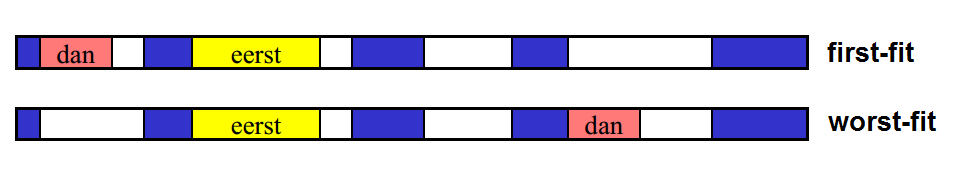
\includegraphics[width=1\textwidth]{geheugenbeheer.png}
		\caption{Schematische weergave van First-fit en Worst-fit}
		\end{center}
	\end{figure}

	\newpage

	\section{Makefile / setup}\label{sec:makefile}
	De makefile maakt twee programma's: worst-fit en first-fit. Om de programma's te maken dient het commando 'make' uitgevoerd te worden. De programma's worden dan gecompileerd en gelinkt. Om beide programma's snel achter elkaar te runnen moet eerst de directory 'out' worden gemaakt. Dit kan door middel van het commando 'make setup' uit te voeren. Vervolgens worden doormiddel van het commando 'make run' beide programma's uitgevoerd. De input die aan de programma's meegegeven wordt staat in de file 'input.txt' in de directory 'input'. De output die het programma geeft wordt weggeschreven naar 'worst-fit.txt' of 'first-fit.txt' in de directory out. Om de output snel te verwijderen kan het commando 'make cleanout' worden uitgevoerd. De uitvoer bestanden worden dan verwijderd. Om alle gecompileerd en gelinkt files te verwijderen kan het commando 'make clean' gebruikt worden. Om zowel de outputfiles als de gecompileerde en gelinkte files te verwijderen kan het commando 'make cleanall' gebruikt worden.

	\section{Het programma}\label{sec:programma}	
		\subsection{Blok administratie}\label{sec:programmablok}
			In het programma wordt gebruik gemaakt van een administratie die vooraan het geheugenblok geplaatst is. Dit administratieblok bestaat uit vier delen:
			\begin{itemize}
				\item De lengte van het geheugenblok
				\item De index van het administratieblok van het vorige geheugenblok
				\item De index van het administratieblok van het volgende geheugenblok
				\item De status van het geheugenblok, is deze vrij of bezet.
			\end{itemize}
			Al deze delen worden in het geheugen gerepresenteerd als 16 bit shorts. het totale administratieblok is dus 64 bits.
			Het programma is zelf in staat om te ontdekken op wat voor machine het draait.
			Als het programma op een 32 bits machine draait zal het programma mem-access-32.c gebruiken.
			Hierin wordt het administratieblok als twee 32 bits longs gerepresenteerd.
			Als het programma op een 64 bits machine gedraaid wordt zal het automatisch mem-access-64.c gebruiken.
			Dit zorgt er voor dat het gehele administratieblok in een 64 bits long geplaatst word.
		
		\subsection{Globale administratie}\label{sec:programmaglobaal}
			Het programma moet ook kunnen bijhouden hoeveel geheugen het heeft toegewezen en hoeveel loze ruimte er gebruikt is.
			Hiervoor gebruikt het programma de eerste twee longs. De allereerste long bevat het aantal toegewezen woorden.
			De tweede long bevat het aantal loze woorden, dit is het aantal woorden dat gebruikt wordt voor de administratie van de blokken.
			De eerste twee longs zelf worden niet als loze woorden gerekend.
			Er is expliciet gekozen om deze twee administratie items niet samen te voegen tot een long aangezien dit de toegang tot deze administratie veel lastiger maakt.
			Aangezien de eerste twee longs altijd gebruikt worden kunnen deze nooit in een blok voorkomen.
			Het eerste vrij blok dat de gehele ruimte omvat is dus de lengte van het geheugen min 2 min de blok administratie lengte.
		
		\subsection{Blok functies}\label{sec:programmafunc}
			Voor het gemak zijn de functies die blokken wijzigen gescheiden van het programma zelf. Er zijn 3 functies die gebruikt worden door beide programma's.
			De eerste functie is new\_block, deze functie maakt een nieuw blok aan met aangegeven lengte. De tweede functie is de split\_block functie, deze functie
			probeert geheugen toe te wijzen door een gegeven blok op te delen in twee nieuwe blokken. Het eerste blok zal dan de hoeveelheid gevraagd geheugen bevatten
			en het tweede blok bevat de overgebleven vrije ruimte. Als er geen ruimte meer overblijft voor een tweede blok zal simpelweg het gehele blok toegewezen worden.
			De laatste functie is free\_block, deze functie zal een blok op een gegeven index vrij geven.
			Als er omringende blokken ook vrij zijn zal het blok samengevoegd worden met die blokken tot een groot nieuw vrij blok.
			
		\subsection{Het first-fit programma}\label{sec:programmaff}
			Het first fit programma is zo gemaakt dat het bij een aanvraag van een stuk geheugen over de blokken zal gaan lopen.
			Het programma begint bij het blok op index 2, aangezien 0 en 1 gebruikt worden voor globale administratie.
			Als het blok op index 2 niet vrij is of niet groot genoeg zal het blok kijken naar het blok op de index gegeven bij de volgende index in
			de administratie van het blok op index 2. Dit gaat zo door tot een geschikt blok gevonden is.
			Hierna zal het programma als het blok precies groot genoeg is het blok toewijzen.
			Als het blok groter is dan de aanvraag wordt de split\_block functie gebruikt.
			Als er geen geschikt blok gevonden is zal de aanvraag geweigerd worden.
			
		\subsection{Het worst-fit programma}\label{sec:programmawf}
			Het worst fit programma komt in grote delen overeen met het first fit programma.
			Het verschil is dat het programma alle blokken af loopt en het grootste vrije gat zoekt.
			Als het programma een blok tegen komt dat precies groot genoeg is stopt hij de zoektocht en wijst het toe.
			Anders zal het grootst gevonden blok gesplit worden met de split\_block functie.
			Als er geen geschikt blok is gevonden zal de aanvraag geweigerd worden.

	\newpage

	\section{Resultaten}\label{sec:resultaten}
	\subsection{Uitvoer first-fit}\label{sec:uitvoerff}
	Aanroep van `mem\_init'\\
ARCH: 2\\
Terug uit `mem\_init'\\
Wil je de `pre\_test' functie overslaan (ja/nee)? [nee]?Aanroep van `pre\_test'\\
Filling up memory\\
Grootste gat = 32764	 vraag aan 16382 -- toegewezen op 4\\
Grootste gat = 16380	 vraag aan 8190 -- toegewezen op 16388\\
Grootste gat = 8188	 vraag aan 4094 -- toegewezen op 24580\\
Grootste gat = 4092	 vraag aan 2046 -- toegewezen op 28676\\
Grootste gat = 2044	 vraag aan 1022 -- toegewezen op 30724\\
Grootste gat = 1020	 vraag aan 510 -- toegewezen op 31748\\
Grootste gat = 508	 vraag aan 254 -- toegewezen op 32260\\
Grootste gat = 252	 vraag aan 126 -- toegewezen op 32516\\
Grootste gat = 124	 vraag aan 62 -- toegewezen op 32644\\
Grootste gat = 60	 vraag aan 30 -- toegewezen op 32708\\
Grootste gat = 28	 vraag aan 14 -- toegewezen op 32740\\
Grootste gat = 12	 vraag aan 6 -- toegewezen op 32756\\
Grootste gat = 4	 vraag aan 2 -- toegewezen op 32764\\
Terug uit `pre\_test'\\
Gebruikte random seed 10\\
Terug uit `init\_test'\\
Terug uit `init\_stats'\\
Geef het aantal samples per test (10 tot 1000) :testgrootte = 1000\\
\\
uniforme random-verdeling van blok-grootten\\
\\
\\
Gemiddelden over 1000 aanvragen:\\
Toegewezen: 426 ; Geweigerd: 574\\
De gemiddelde grootte van de toegewezen aanvragen is 11180.1\\
De gemiddelde grootte van de geweigerde aanvragen is 20508.1\\
Het experiment liep over 332.639784 gesimuleerde tijdseenheden\\
Gemiddeld over deze gesimuleerde tijd waren er - \\
 18037.5 woorden geheugen in gebruik\\
 14727.2 woorden geheugen vrij\\
     3.3 woorden geheugen in fragmenten\\
Er waren gemiddeld     1.64 stukken geheugen toegewezen (max 5, min 0)\\
Er waren gemiddeld     1.42 gaten, met een maximum van 3 en een minimum van 1\\
\\
Histogram van de aantallen toegewezen en geweigerde aanvragen\\
tegen de grootte van de aanvraag (per 512 woorden):\\
\begin{center}
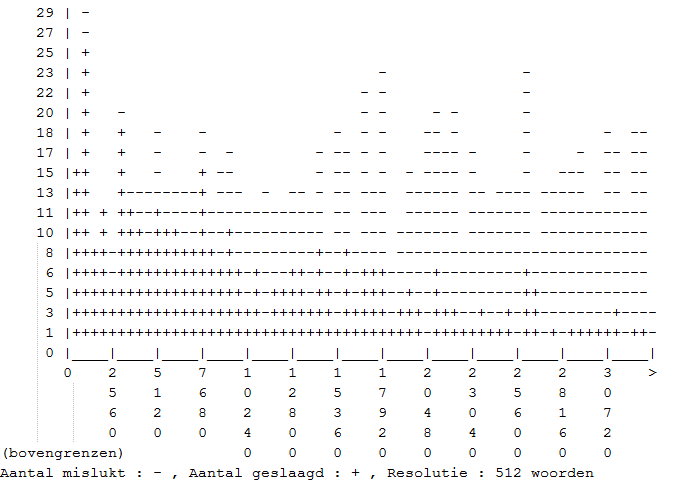
\includegraphics[width=0.8\textwidth]{ff1.png}
\end{center}
Histogram van de totale tijdsduur dat het grootste gat een\\
bepaalde omvang had tegen de grootte van dat gat(per 512 woorden):
\begin{center}
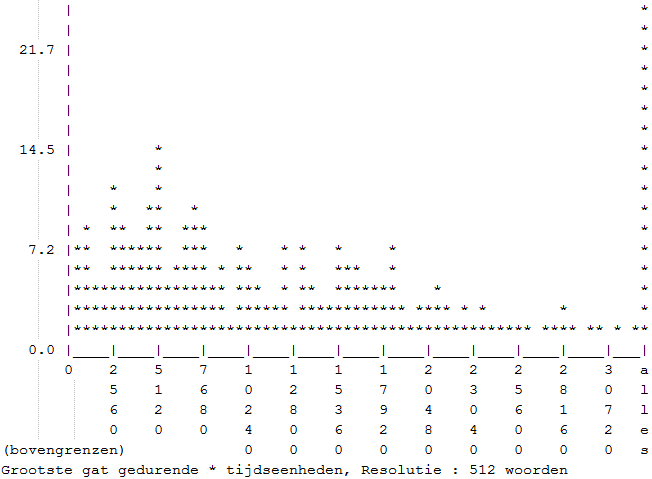
\includegraphics[width=0.8\textwidth]{ff2.png}
\end{center}
exponentiele random-verdeling van blok-grootten\\
\\
\\
Gemiddelden over 1000 aanvragen:\\
Toegewezen: 655 ; Geweigerd: 345\\
De gemiddelde grootte van de toegewezen aanvragen is 2034.2\\
De gemiddelde grootte van de geweigerde aanvragen is 6957.2\\
Het experiment liep over 331.195869 gesimuleerde tijdseenheden\\
Gemiddeld over deze gesimuleerde tijd waren er - \\
 23396.5 woorden geheugen in gebruik\\
  9348.1 woorden geheugen vrij\\
    23.4 woorden geheugen in fragmenten\\
Er waren gemiddeld    11.64 stukken geheugen toegewezen (max 19, min 6)\\
Er waren gemiddeld     5.90 gaten, met een maximum van 11 en een minimum van 3\\
\\
Histogram van de aantallen toegewezen en geweigerde aanvragen\\
tegen de grootte van de aanvraag (per 512 woorden):
\begin{center}
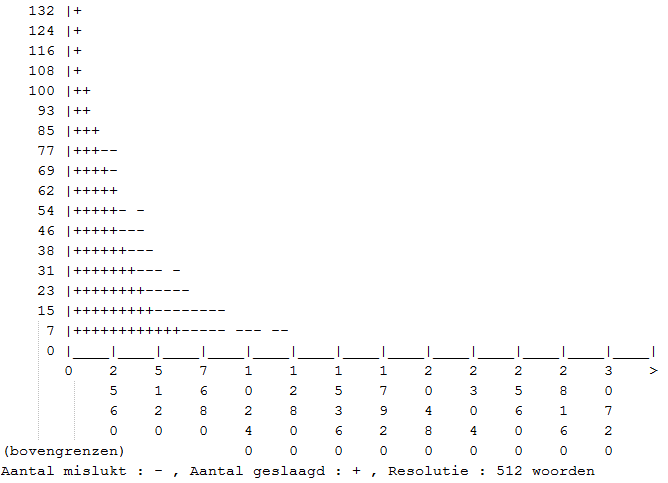
\includegraphics[width=0.8\textwidth]{ff3.png}
\end{center}
Histogram van de totale tijdsduur dat het grootste gat een\\
bepaalde omvang had tegen de grootte van dat gat(per 512 woorden):
\begin{center}
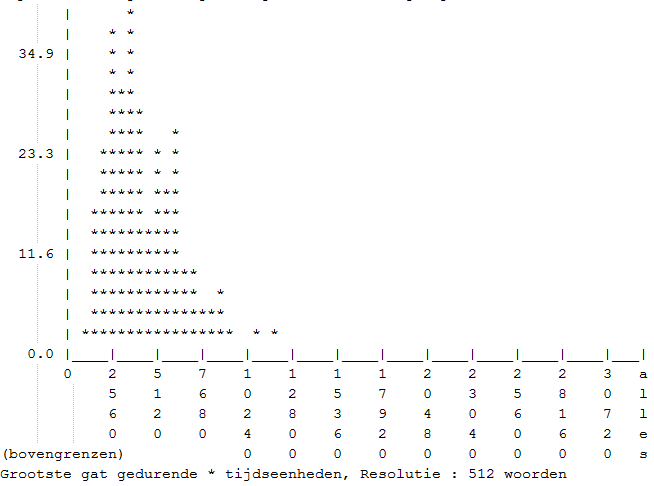
\includegraphics[width=0.8\textwidth]{ff4.png}
\end{center}
kwadratische random-verdeling van blok-grootten\\
\\
\\
Gemiddelden over 1000 aanvragen:\\
Toegewezen: 590 ; Geweigerd: 410\\
De gemiddelde grootte van de toegewezen aanvragen is 5144.7\\
De gemiddelde grootte van de geweigerde aanvragen is 19419.9\\
Het experiment liep over 341.737404 gesimuleerde tijdseenheden\\
Gemiddeld over deze gesimuleerde tijd waren er - \\
 17503.8 woorden geheugen in gebruik\\
 15257.4 woorden geheugen vrij\\
     6.8 woorden geheugen in fragmenten\\
Er waren gemiddeld     3.42 stukken geheugen toegewezen (max 9, min 0)\\
Er waren gemiddeld     2.17 gaten, met een maximum van 4 en een minimum van 1\\
\\
Histogram van de aantallen toegewezen en geweigerde aanvragen\\
tegen de grootte van de aanvraag (per 512 woorden):
\begin{center}
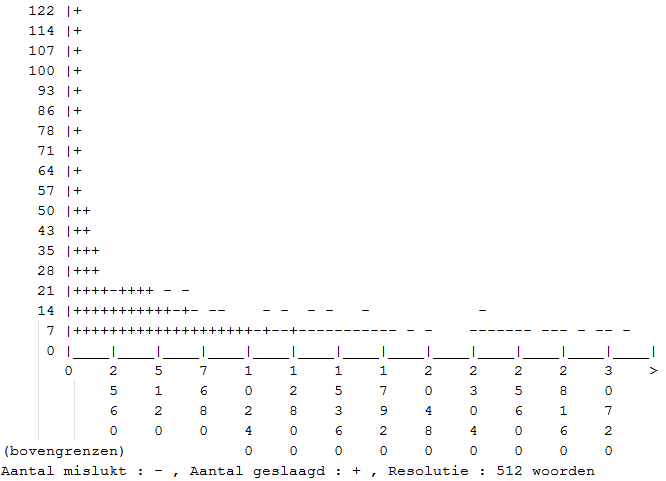
\includegraphics[width=0.8\textwidth]{wf5.png}
\end{center}
Histogram van de totale tijdsduur dat het grootste gat een\\
bepaalde omvang had tegen de grootte van dat gat(per 512 woorden):
\begin{center}
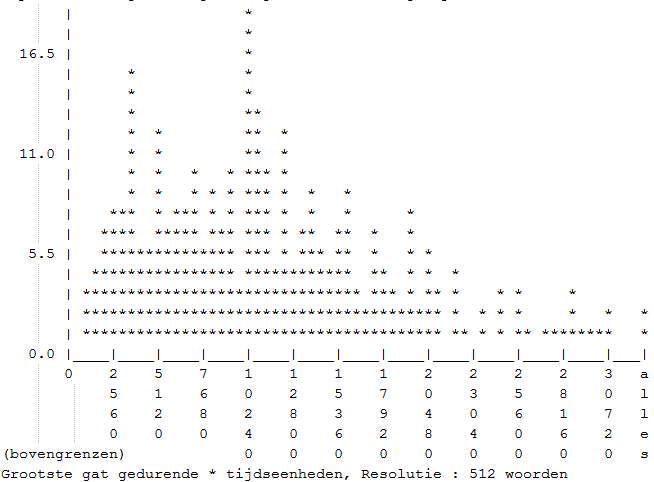
\includegraphics[width=0.8\textwidth]{ff6.png}
\end{center}

\newpage

	\subsection{Uitvoer worst-fit}\label{sec:uitvoerwf}
Aanroep van `mem\_init'\\
Terug uit `mem\_init'\\
Wil je de `pre\_test' functie overslaan (ja/nee)? [nee]?Aanroep van `pre\_test'\\
Filling up memory\\
Grootste gat = 32764	 vraag aan 16382 -- toegewezen op 4\\
Grootste gat = 16380	 vraag aan 8190 -- toegewezen op 16388\\
Grootste gat = 8188	 vraag aan 4094 -- toegewezen op 24580\\
Grootste gat = 4092	 vraag aan 2046 -- toegewezen op 28676\\
Grootste gat = 2044	 vraag aan 1022 -- toegewezen op 30724\\
Grootste gat = 1020	 vraag aan 510 -- toegewezen op 31748\\
Grootste gat = 508	 vraag aan 254 -- toegewezen op 32260\\
Grootste gat = 252	 vraag aan 126 -- toegewezen op 32516\\
Grootste gat = 124	 vraag aan 62 -- toegewezen op 32644\\
Grootste gat = 60	 vraag aan 30 -- toegewezen op 32708\\
Grootste gat = 28	 vraag aan 14 -- toegewezen op 32740\\
Grootste gat = 12	 vraag aan 6 -- toegewezen op 32756\\
Grootste gat = 4	 vraag aan 2 -- toegewezen op 32764\\
Terug uit `pre\_test'\\
Gebruikte random seed 10\\
Terug uit `init\_test'\\
Terug uit `init\_stats'\\
Geef het aantal samples per test (10 tot 1000) :testgrootte = 1000\\
\\
uniforme random-verdeling van blok-grootten\\
\\
\\
Gemiddelden over 1000 aanvragen:\\
Toegewezen: 425 ; Geweigerd: 575\\
De gemiddelde grootte van de toegewezen aanvragen is 11087.4\\
De gemiddelde grootte van de geweigerde aanvragen is 20560.4\\
Het experiment liep over 332.639784 gesimuleerde tijdseenheden\\
Gemiddeld over deze gesimuleerde tijd waren er - \\
 17902.1 woorden geheugen in gebruik\\
 14862.6 woorden geheugen vrij\\
     3.3 woorden geheugen in fragmenten\\
Er waren gemiddeld     1.64 stukken geheugen toegewezen (max 5, min 0)\\
Er waren gemiddeld     1.43 gaten, met een maximum van 3 en een minimum van 1\\
\\
Histogram van de aantallen toegewezen en geweigerde aanvragen\\
tegen de grootte van de aanvraag (per 512 woorden):
\begin{center}
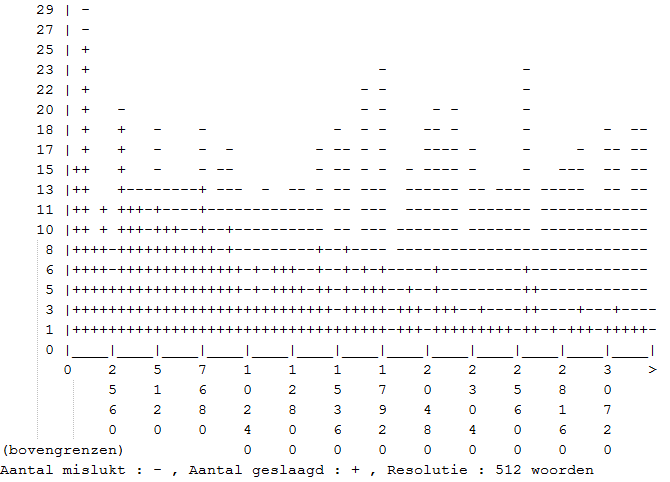
\includegraphics[width=0.8\textwidth]{wf1.png}
\end{center}
Histogram van de totale tijdsduur dat het grootste gat een\\
bepaalde omvang had tegen de grootte van dat gat(per 512 woorden):
\begin{center}
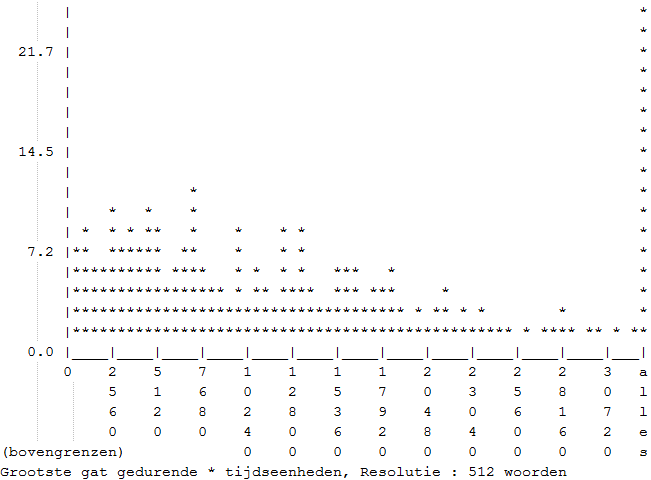
\includegraphics[width=0.8\textwidth]{wf2.png}
\end{center}
exponentiele random-verdeling van blok-grootten\\
\\
\\
Gemiddelden over 1000 aanvragen:\\
Toegewezen: 641 ; Geweigerd: 359\\
De gemiddelde grootte van de toegewezen aanvragen is 1887.7\\
De gemiddelde grootte van de geweigerde aanvragen is 7026.9\\
Het experiment liep over 331.195869 gesimuleerde tijdseenheden\\
Gemiddeld over deze gesimuleerde tijd waren er - \\
 20817.4 woorden geheugen in gebruik\\
 11927.9 woorden geheugen vrij\\
    22.7 woorden geheugen in fragmenten\\
Er waren gemiddeld    11.36 stukken geheugen toegewezen (max 19, min 6)\\
Er waren gemiddeld     5.83 gaten, met een maximum van 10 en een minimum van 3\\
\\
Histogram van de aantallen toegewezen en geweigerde aanvragen\\
tegen de grootte van de aanvraag (per 512 woorden):
\begin{center}
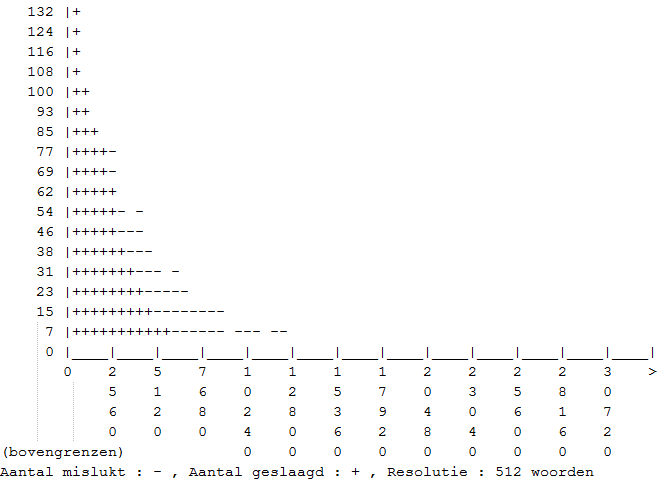
\includegraphics[width=0.8\textwidth]{wf3.png}
\end{center}
Histogram van de totale tijdsduur dat het grootste gat een\\
bepaalde omvang had tegen de grootte van dat gat(per 512 woorden):
\begin{center}
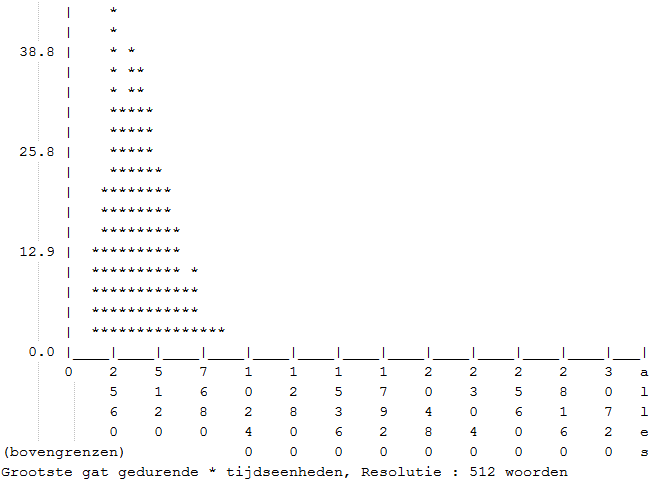
\includegraphics[width=0.8\textwidth]{wf4.png}
\end{center}
kwadratische random-verdeling van blok-grootten\\
\\
\\
Gemiddelden over 1000 aanvragen:\\
Toegewezen: 583 ; Geweigerd: 417\\
De gemiddelde grootte van de toegewezen aanvragen is 4840.5\\
De gemiddelde grootte van de geweigerde aanvragen is 19605.6\\
Het experiment liep over 341.737404 gesimuleerde tijdseenheden\\
Gemiddeld over deze gesimuleerde tijd waren er - \\
 16677.8 woorden geheugen in gebruik\\
 16083.4 woorden geheugen vrij\\
     6.8 woorden geheugen in fragmenten\\
Er waren gemiddeld     3.39 stukken geheugen toegewezen (max 9, min 0)\\
Er waren gemiddeld     2.23 gaten, met een maximum van 4 en een minimum van 1\\
\\
Histogram van de aantallen toegewezen en geweigerde aanvragen\\
tegen de grootte van de aanvraag (per 512 woorden):
\begin{center}
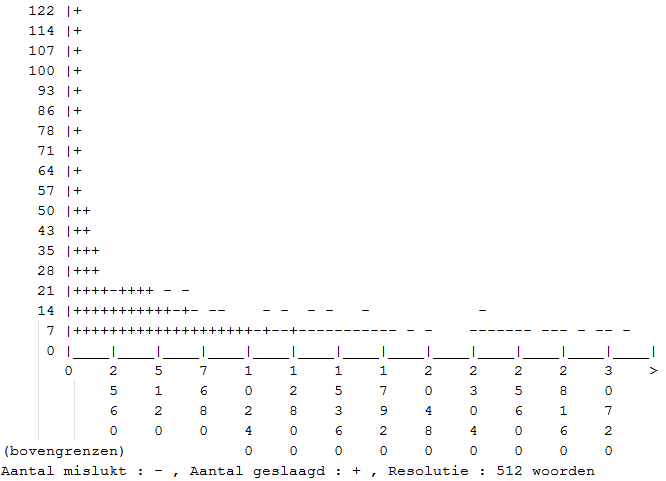
\includegraphics[width=0.8\textwidth]{wf5.png}
\end{center}
Histogram van de totale tijdsduur dat het grootste gat een\\
bepaalde omvang had tegen de grootte van dat gat(per 512 woorden):
\begin{center}
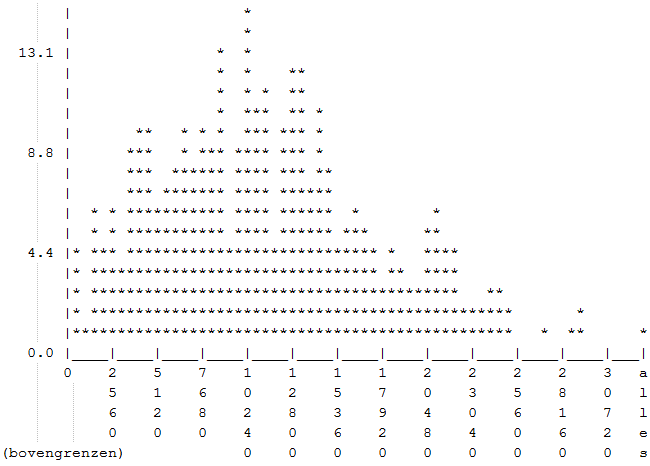
\includegraphics[width=0.8\textwidth]{wf6.png}
\end{center}
Grootste gat gedurende * tijdseenheden, Resolutie : 512 woorden
\newpage

	\section{Vergelijking}\label{sec:vergelijking}
	De vergelijking is gebaseerd op de resultaten als gegeven in resultaten(\ref{sec:resultaten}).

	\subsection{Uniforme random-verdeling}\label{sec:urv}
	Bij de uniforme random-verdeling van blok-grootten zijn er nauwelijks verschillen tussen first-fit en worst-fit. First-fit krijgt \'e\'en aanvraag meer toegewezen, namelijk 426, ten opzichte van worst-fit. First-fit heeft een hoger gemiddeld aantal woorden in gebruik, 18037.5 tegen 17902.1. De gemiddelde grootte van een aanvraag is bij first-fit ook iets groter, 11180.1 tegen 11087.4. First-fit had vaker kleine gaten als grootste gat. First-fit presteerde net iets beter, maar de verschillen zijn echter zo klein dat worst-fit hier ook goed presteerd.

	\subsection{Exponentiele random-verdeling}\label{sec:erv}
	De verschillen bij de exponentiele random-verdeling van blok-grootten zijn al groter dan bij de uniforme random-verdeling(\ref{sec:urv}). Bij first fit worden 655 aanvragen toegewezen tegen 641 bij worst-fit. First-fit heeft gemiddeld 23396.5 woorden in gebruik tegen 20817.4 bij worst-fit. First-fit wist ook enkele grotere aanvragen te behandelen waardoor de gemiddelde grootte van een aanvraag hoger ligt dan die van worst fit, 2034.2 tegen 1887.7. First-fit hield over het algemeen grote gaten langer vrij dan worst-fit. First-fit presteert beduidend beter. Er werden vaker aanvragen toegewezen dan bij worst-fit. Waarschijnlijk komt dit vooral omdat grote aanvragen bij first-fit wel toegewezen kunnen worden, omdat er vaker grote gaten beschikbaar zijn, en bij worst-fit niet.

	\subsection{Kwadratische random-verdeling}\label{sec:krv}
	Bij de kwadratische random-verdeling worden bij first-fit 590 aanvragen toegewezen tegen 583 aanvragen bij worst-fit. Gemiddeld had first-fit 17503.8 woorden in gebruik tegen 16677.8 woorden bij worst-fit. Worst-fit weet vaker grotere aanvragen af te handelen. First-fit handelt echter veel vaker middelgrote aanvragen af. Dit resulteert in een hoger gemiddelde per aanvraag voor first-fit, 5144.7 tegen 4840.5. First-fit heeft vaker hele grote grootste gaten dan worst-fit. Worst-fit heeft echter vaker grootste gaten bij middelgrote aanvragen. Al met al werkt first-fit hier het beste, omdat er vaker aanvragen worden toegewezen en elke aanvraag gemiddeld groter is dan bij worst-fit.

\newpage

	\subsection{Conclusie}
	Bij elke test komt first-fit als beste algoritme naar voren. Waar het verschil bij de uniforme random-verdeling(\ref{sec:urv}) nog niet zo groot was werden de verschillen bij de exponentiele random-verdeling(\ref{sec:erv}) en de kwadratische random-verdeling(\ref{krv}) alleen maar groter. First-fit wees vaker aanvragen toe. Daarnaast waren de gemiddelde groottes per aanvraag bij first-fit groter, wat betekent dat ook grotere aanvragen bij first-fit vaker worden toegewezen. Worst-fit presteert nog wel goed, maar first-fit is overduidelijk beter.

\end{document}
